\documentclass{article}

%............Inicia Preambulo.......................
\usepackage{graphicx}
\usepackage{float}
\usepackage[utf8]{inputenc}
\usepackage[shortlabels]{enumitem}
\usepackage{textcomp}
\usepackage{multicol}
\usepackage{caption}
\usepackage[spanish]{babel}
\usepackage[total={17.5cm, 23cm}, top=2cm, left=2cm]{geometry}
\usepackage{esvect}
\usepackage[font=footnotesize]{caption}

\spanishdecimal{.}
\parindent 0cm

%.............Fin de Preambulo........................

\begin{document}

\begin{center}
{\Large \textbf{Universidad Autónoma de Coahuila}}
\end{center}

\begin{center}
{\large Facultad de Ciencias Físico-Matemáticas}
\end{center}

%Materia
\begin{center}
{\large Metodos Numericos}
\end{center}

%Título
\begin{center}
{\large Regla Falsa}
\end{center}

%Fecha
\begin{center}
{\large 29 de Noviembre del 2019}
\end{center}

%Autor
\begin{center}
{\large José Antonio Olveda García}
\end{center}

\vspace{5mm}

\begin{multicols}{2}

\section{Objetivo}
\label{sec:obj}
  Mostrar la utilidad del buscador de raices de polinomios por medio del metodo de regla falsa, asi como las ventajas y desventajas que este pueda presentar

\section{Introducción}
\label{sec:intro}
Es una mezcla de la seguridad del metodo de biseccion con la rapidez del metodo de la secante, que mide los puntos con una recta que intersecta en el eje x, la cual proporciona una mejor aproximacion a la raiz.
\\
Reemplazamiento de la curva por una recta de una posicion falsa de la raiz.
\section{Metodologia}
\label{sec:Met}
El método de la regla falsa, o "falsa posición", es otro de los muchos métodos iterativos para la resolución de problemas con ecuaciones no lineales. La peculiaridad de éste, es que combina dos métodos: el método de bisección y el de la secante (ya explicados en otros artículos).

A continuación veremos una explicación de en qué consiste.
\\
Se basa en trazar una recta que una los extremos de un intervalo dado, considerando que la solución está cerca de uno de éstos extremos.

Hemos agregado por tanto, esa línea recta que une el intervalo [a,b]. La idea principal es que si tomamos el punto donde la recta corta el eje x, estaremos más cerca de hallar la raíz.

Entonces, supongamos que tenemos una función f(x), que es continua en el intervalo $[x_{a}, x_{b}]$, y que además $f(x_{a})$ y $f(x_{b})$ tienen signos opuestos por lo que se deduce que existe al menos una solución para esa ecuación.


 
Ahora, necesitamos saber la ecuación de la línea recta que une esos dos puntos. Para ello nos ayudamos de la ecuación punto-pendiente, por eso, hallamos la pendiente:
\begin{equation}
m=\frac{f(x_{a})-f(x_{b})}{x_{b}-x_{a}}
\end{equation}
Ahora vamos a sustituir eso en la ecuación de la recta:
\begin{equation}
y-f(x_{a})=\frac{f(x_{a})-f(x_{b})}{x_{b}-x_{a}} (x-x_{a})
\end{equation}
Simplificamos multiplicando todo por xb-xa, para quitar el denominador:
\begin{equation}
(y-f(x_{a}))(x_{b}-x_{a})=f(x_{a})-f(x_{b})(x-x_{a})
\end{equation}
Como paso final, despejamos la incógnita x:
\begin{equation}
x=x_{a}-\frac{f(x_{a})(x_{b}-x_{a})}{f(x_{b})-f(x_{a})}
\end{equation}
Vamos ahora a describir paso a paso como se desarrolla el método de la regla falsa (considerando f(x) continua):

1) Primero debemos encontrar unos valores iniciales xa y xb tales que:
\begin{equation}
f(x_{a})f(x_{b})<0
\end{equation}
2) Aproximamos a la raíz, para ello usamos la ecuacion 4.
\\
3) Evaluamos $f(x_{r})$. Se pueden dar hasta tres casos:
\begin{center}
$f(x_{a})f(x_{r})<0$
\end{center}
Como $f(x_{a})$ y $f(x_{r})$ tienen signos opuestos, por la condición mencionada anteriormente deducimos que, la raíz se encuentra en el intervalo $[x_{a}, x_{r}]$

B)
\begin{center}
$f(x_{a})f(x_{r})>0$
\end{center}


$f(x_{a})$ y $f(x_{r})$ tienen el mismo signo. Así que $x_{b}$ y $x_{r}$ han de tener signos distintos, pues:

\begin{center}
$f(x_{r})f(x_{b})<0$
\end{center}


Por tanto, la raíz se encuentra en el intervalo $[x_{r}, x_{a}]$.

Como consideramos que la ecuación tiene que ser continua (si o si), al darse este caso, no cumpliría con la condición de continuidad, al menos que tomemos como referencia un tercer punto $(x_{r})$ cuya imagen $(f(x_{r}))$ será de signo opuesto.
\\
C)
\begin{center}
$f(x_{a})f(x_{r})=0$
\end{center}


En este caso, como $f(x_{r})=0$ ya tenemos localizada la raíz.

 

Debemos repetir estos 3 pasos señalados anteriormente hasta que:

$|Ea|<Eb$
\section{Ejemplo}
\label{sec:Ejem}
Resuelva el siguiente polinomio por medio de la regla falsa.
\begin{center}
$2x^{4}-5^{2}+x $ en el intervalo $[1,3.5]$
\end{center}
Evaluando obtenemos los siguientes valores
\\
$f_{a}=-2$ 
\\
$f_{b}=242.3$
\\
$x_{a}=1$
\\
$x_{b}=3.5$
Aplicando la regla falsa obtenemos que el punto de la primera aproximacion es de 
$c=4.502$
Realizando la multiplicacion entre las funciones evaluadas en a y c, obtenemos 
\begin{center}
$-2*4.502=-9.004$
\end{center}
Por lo tanto se extiende la regla ahora con un nuevo intervalo, siendo de $[4,502,3.5]$, volviendo a realizar la regla falsa obtenemos un valor de $c=2.9$, extiendose la comprobacion has $n$ iteraciones deseadas.
Graficado por medio de Geogebra obtenemos una de sus raices la cual es $x=1.674$
\begin{figure}[H]
\centering
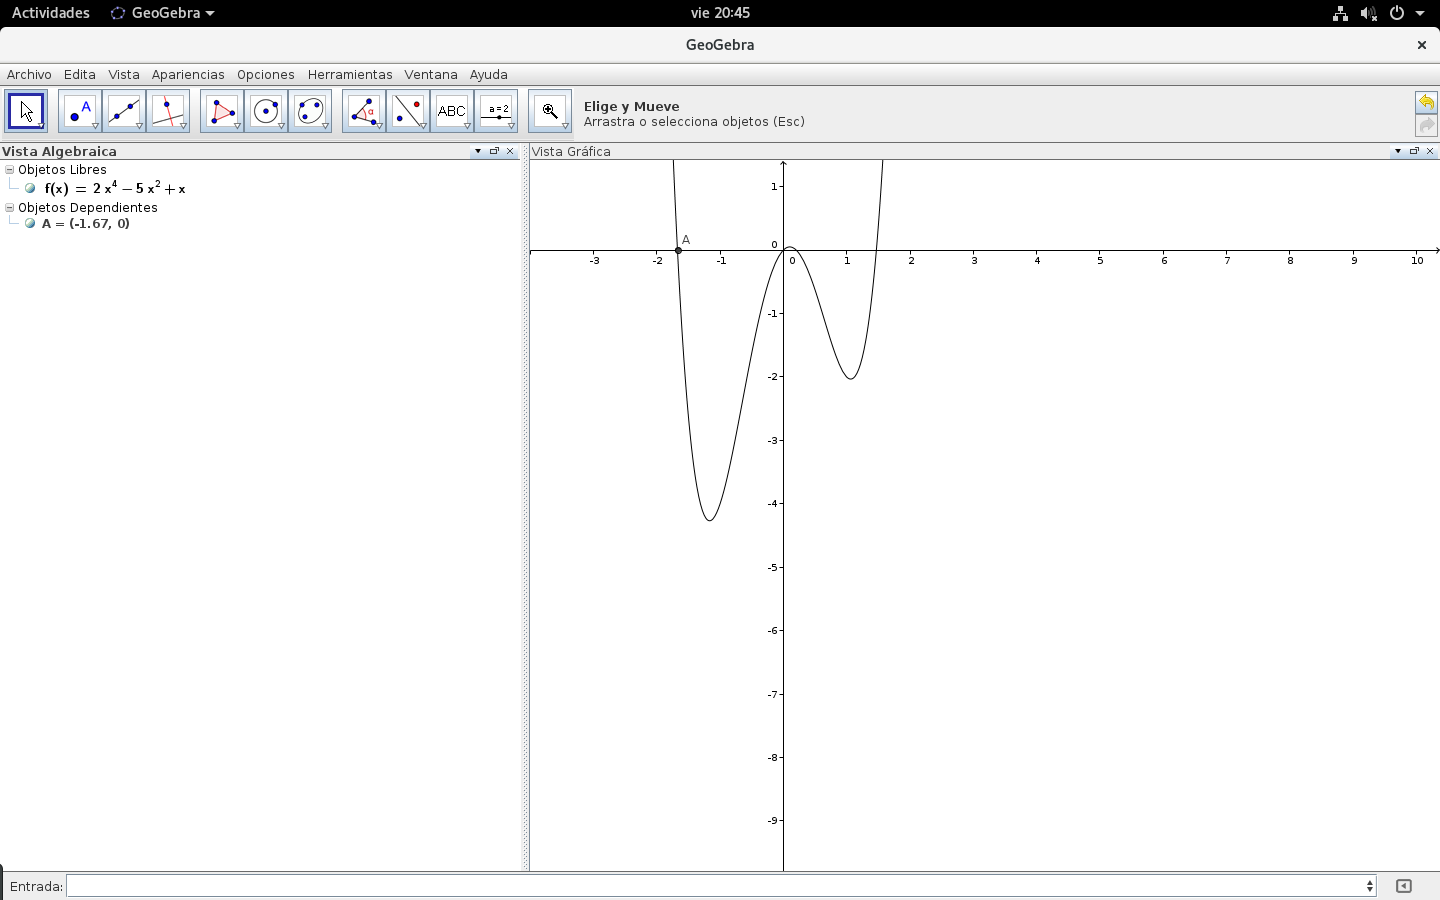
\includegraphics[scale=.125]{GeogebraFalso.png}
\caption{Programa del metodo de Regla Falsa}
\end{figure}

\section{Ventajas y Desventajas}
\textbf{Ventajas}
\\
1. La ventaja del método de Regla - Falsa, al igual que el de bisección, es que es siempre convergente para funciones continuas f(x). Aunque en general, converge más rápidamente que el método de la bisección.
\\
\\
\textbf{Desventajas}
\\
1. Converge lentamente a la solucion, debido al efectuar las iteraciones uno de las extremos del intervalo no se modifica.
\section{Implementacion del programa}
\label{sec:Imp}
El proceso de regla falsa al ser tan similar al de biseccion, lo unico que se genero un cambio considerable en el fue la declaracion de la nueva ecuacion establecida por regla falsa, manteniendo los demas factores ingresados dentro de estos
\begin{figure}[H]
\centering
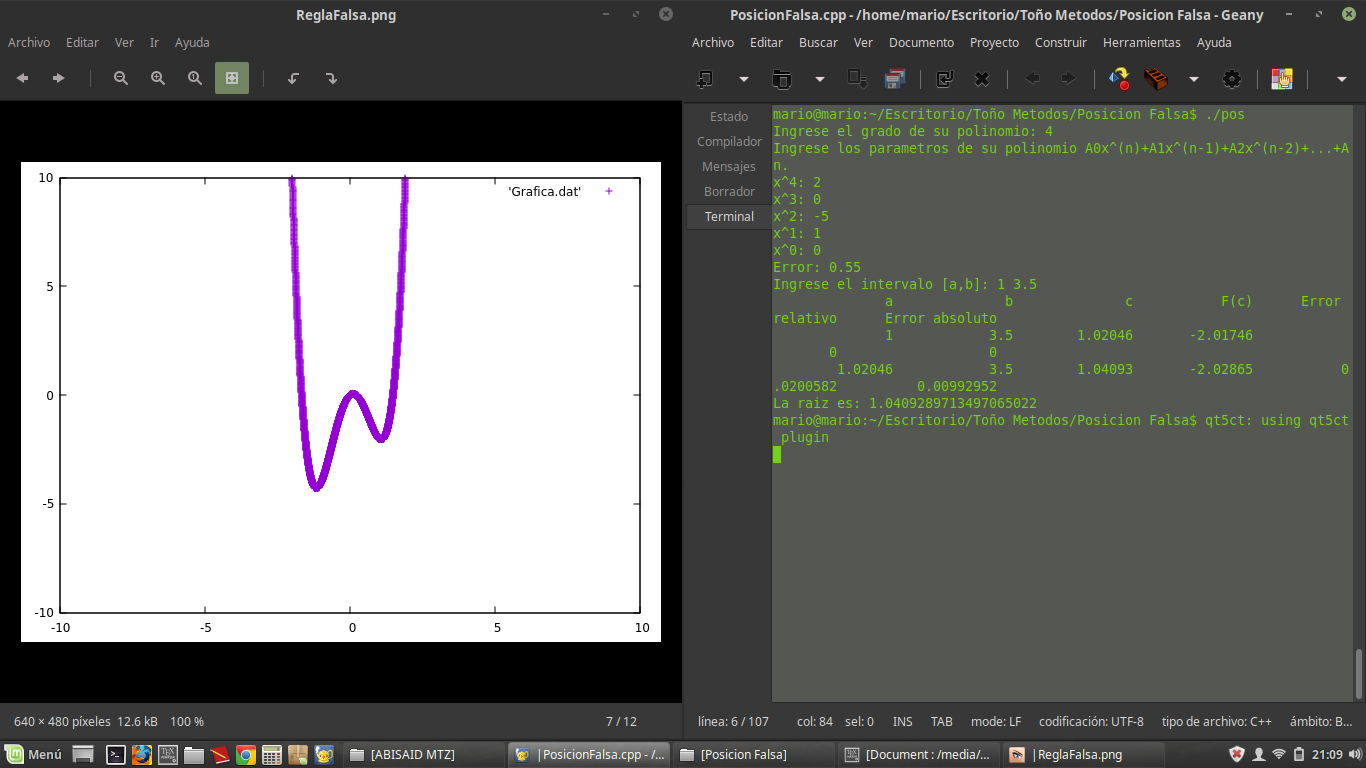
\includegraphics[scale=.125]{ReglaFalsa.png}
\caption{Programa del metodo de Regla Falsa}
\end{figure}
como podemos analizar de la situacion la raiz de corte nos dio un valor de $x=1.04$ siendo bastante aproximado al metodo implementado

\end{multicols}

\end{document}
